\metadata{16}{Leah Reeder and Trevor Maxfield}{Nov 10th, 2021}

\sec{From small to large initialization: a precise characterization}

We have previously discussed how certain initializations of gradient descent converge to minimum-norm solutions. In the sequel, we characterize the effect of initialization more precisely---we will show that in a variant of the settings in Section~\ref{sec:small_init_nonlinear}, we can precisely compute the corresponding regularizer induced by any initialization. We will see that when the initialization is small, we obtain the bias towards minimum norm solution (in the parameter space used in optimization), whereas when the initialization is large, we are in the NTK regime (Section~\ref{sec:ntk_approach}) where the implicit bias is towards the min norm solution under the NTK kernel. The materials in this subsection are simplifications of results in the recent paper~\citet{woodworth2020kernel}.

\subsection{Preparation: gradient flow}
To simplify the analysis, we will consider the concept of gradient flow, i.e. gradient descent with an infinitesimal learning rate.  This allows us omit the second order effect from the learning rate and simplify the analysis. 

We begin by recalling the gradient descent update formula. In our previous description of gradient descent, we indexed the updated parameters by $t = 1,2,\dots$. Anticipating our generalization to infinitesimal steps, we will index the updated parameters using parentheses instead of subscripts. In particular, the standard gradient descent update given a loss function $L(w)$ is
\al{
w(t+1) = w(t) - \eta \nabla L(w(t)).
}
If we scale the time by $\eta$ so that each update by gradient descent corresponds to a time step of size $\eta$ (rather than size 1), the update becomes
\al{
w(t + \eta) = w(t) - \eta \nabla L(w(t)).
}
Taking $\eta \to 0$ yields a differential equation, which can be thought of as a continuous process rather than discrete updates:
\al{
w(t+dt) = w(t) - dt \cdot \nabla L(w(t)).
}
This can also be written as:
\al{
\dot{w}(t) = -\nabla L(w(t) \quad \text{ with } \quad \dot{w}(t) = \frac{\partial w(t)}{\partial t}
}
This allows us to ignore the $\eta^2$ term (alternatively the $(dt^2)$ term), which will simplify some of the technical details that follow.

\subsec{Characterizing the implicit bias of initialization}
The results in this section are slight simplification of the recent paper by~\citet{woodworth2020kernel}. The model is a variant of the one we introduced in \eqref{lec13:eqn:hadamard_model_1}. Recalling that $x^{\odot 2} = x \odot x$, let
\al{
f_w(x) = \left(w_+^{\odot 2} - w_-^{\odot 2}\right)^\top x.
}
where $w_+, w_- \in \R^d$. Let $w$ denote the concatenation of the two parameter vectors, i.e. $= (w_+, w_-)$.  In \eqref{lec13:eqn:hadamard_model_1}, we defined $f_\beta(x) = (\beta \odot \beta)^\top x$; this model can only represent positive linear combinations of $x$.  By contrast, $f_w(x)$ can represent any linear model. Moreover, if we choose our initialization for $w$ such that $w_+(0) = w_-(0)$, we obtain $f_{w(0)}(x) \equiv 0$ for all $x$. Similar to our analysis of the NTK, this initialization will simplify the subsequent derivations.

Next, we define the following loss function,
\al{
\hatL(w) = \frac{1}{2} \sum_{i=1}^n \left( y\sp{i} - f_w(x\sp{i})\right)^2,
}
and consider the initialization
\al{
w_+(0) = w_-(0) = \alpha \cdot \vec{\mathbf{1}}
}
where $\vec{\mathbf{1}}$ denotes the all-ones vector. The analysis technique still applies to any general initializations as long as all the dimension are initialized to be non-zero, but the the initialization scale is the most important factor, and therefore we chose this simplification for the ease of exposition. 

Note that every $w = (w_+, w_{-})$ corresponds to a de facto linear function of $x$. We denote the resulting linear model as $\theta_w$:
\al{
\theta_w = w_+^{\odot 2} - w_-^{\odot 2}.
}
Note that $\theta_w^\top x = f_w(x)$. 

Let $w(\infty)$ denote the limit of the gradient flow, i.e.
\al{
w(\infty) = \lim_{t \to \infty} w(t).
}
Then, the converged linear model in the $\theta$ space is defined by $\theta_\alpha(\infty) = \theta_{w(\infty)}$---we are interested in understanding its properties.  For simplicity, we will omit the $\infty$ index and refer to this quantity as $\theta_\alpha$. We assume throughout that the limit exists and all corresponding regularity conditions are met.

Let
\al{
X = \begin{bmatrix} x^{(1)^\top} \\ \vdots \\ x^{(n)^\top} \end{bmatrix} \in \R^{n \times d} \quad \text{ and } \quad \vec{y} = \begin{bmatrix} y^{(1)} \\ \vdots \\ y^{(n)} \end{bmatrix}.
}
In the sequel, we formally state our result relating the complexity of the solution discovered by gradient flow to the size of the initialization.
\begin{theorem}[Theorem 1 in \citet{woodworth2020kernel}]
	 \label{lec16:thm:interpolatingAlpha}
For any $0 < \alpha < \infty$, assume that gradient flow with initialization $w_+(0) = w_-(0) = \alpha \cdot \vec{\mathbf{1}}$ converges to a solution that fits the data exactly: $X \theta_{\alpha} = \vec{y}$.\footnote{This assumption can likely be proved to be true and thus not required. Here we still include the condition because the original paper~\citet{woodworth2020kernel} assumed it.}  Then, the solution satisfies the following notion of minimum complexity:
\al{ 
\theta_\alpha = \argmin_\theta Q_\alpha(\theta)\\
 \quad \textup{ s.t. } \quad X \theta = \vec{y} \label{lec16:eqn:constrained_complexity}
}
where
\al{
Q_\alpha(\theta) = \alpha^2 \cdot \sum_{i=1}^n q\left(\frac{\theta_i}{\alpha^2} \right)
}
and
\al{
q(z) = 2 - \sqrt{4 + z^2} + z \cdot \textup{arcsinh}\left(\frac{z}{2}\right)
}
\end{theorem}
In words, Theorem~\ref{lec16:thm:interpolatingAlpha} claims that $\theta_\alpha$ is the minimum complexity solution for the complexity measure $Q_\alpha$.

%23 minutes.
\begin{remark}
In particular, when $\alpha \to \infty$ we have that 
\begin{align}
    q(\theta_i /\alpha^2) \asymp \theta_i^2/\alpha^4
\end{align}
and so 
\begin{align}
    Q_\alpha(\theta) \asymp \frac{1}{\alpha^2} \Norm{\theta}_2^2.
\end{align}
This means that if $\alpha \to \infty$ than the complexity measure $Q_\alpha$ is the $\ell_2$-norm, $||\theta||_2$.  If $\alpha \to 0$, then the complexity measure becomes
\al{
q\left(\frac{\theta_i}{\alpha^2}\right) &\asymp \frac{\left|\theta_i\right|}{\alpha^2} \log\left(\frac{1}{\alpha^2}\right) \quad\text{(by Taylor expansion)}
}
and so,
\al{
Q_\alpha\left(\theta\right) &\asymp \frac{\Norm{\theta}_1}{\alpha^2} \log\left(\frac{1}{\alpha^2}\right)
}
To summarize, for $\alpha \to \infty$, the constrained minimization problem we solve in \eqref{lec16:eqn:constrained_complexity} yields the minimum $\ell_2$-norm solution of $\theta$ (i.e. the $\ell_4$-norm for $w$).  When $\alpha \to 0$, solving \eqref{lec16:eqn:constrained_complexity} yields the minimum $\ell_1$-norm $\theta$ (which is the $\ell_2$-norm for $w$).  For $0 < \alpha < \infty$, we obtain some interpolation of $\ell_1$ and $\ell_2$ regularization of the optimum.
\end{remark}

%27.30 minutes
\begin{remark}
Note that when $\alpha \to 0$, the intuition is similar to what we had observed in previous analyses; in particular, the solution is the global minimum closest to the initialization.  Note however, that when $\alpha \neq 0$, the solution discovered by gradient descent will not \textit{exactly} correspond to the solution closest to the initialization.
\end{remark}

\begin{remark}
When $\alpha \to \infty$, we claim that the model optimization is in the neural tangent kernel (NTK) regime.  Recall that we had two parameters, $(\sigma, \beta)$, that determined if we could treat the optimization problem as a kernel regression. Further recall that $\sigma$ denotes the minimum singular value of $\Phi$ and $\beta$ is the Lipschitzness of the gradient. Let us now compute $\sigma$ and $\beta$ for large $\alpha$ initializations of our model.

For $w_-(0) = w_+(0) = \alpha \vec{\mathbf{1}}$,
\al{
\nabla f_{w(0)}(x) = 2 \begin{bmatrix} w_{+}(0) \cdot x \\ -w_{-}(0) \odot x \end{bmatrix} = 2 \alpha \begin{bmatrix} x \\ -x \end{bmatrix}
}
by the chain rule.  It is clear then that both $\sigma$ and $\beta$ linearly depend on $\alpha$.  This implies that
\al{
\frac{\beta}{\sigma^2} \to 0 \quad \text{ as } \alpha \to \infty
}
since the denominator is $O(\alpha^2)$, while the numerator is $O(\alpha)$.  In particular, the features used in this kernel method are:
\al{
\phi(x) = \nabla f_{w(0)} (x) = 2 \alpha \begin{bmatrix} x \\ - x \end{bmatrix}
}
The neural tangent kernel perspective then gives an alternative proof of this complexity minimization result for $\alpha \to \infty$. In the NTK regime, the solution (to our convex problem) is always the minimum $\ell_2$-norm solution for the feature matrix, which in this case equals $\begin{bmatrix} X \\ - X \end{bmatrix}$. 

Note that practice tends not to follow the assumptions made here. Often, people either do not use large initializations or do not use infinitesimally small step sizes. But this is a good thing  because we do not want to be in the NTK regime; being in the NTK regime implies that we are doing no different or better than just using a kernel method.
\end{remark}

We can now prove Theorem~\ref{lec16:thm:interpolatingAlpha}, which is similar to the overparametrized linear regression proof of Theorem~\ref{lec13:thm:linear-main}.

This proof follows in two steps:
\begin{enumerate}
\item We find an invariance maintained by the optimizer. In the overparametrized linear regression proof of Theorem~\ref{lec13:thm:linear-main}, we required $\theta \in \text{span}\{x\sp{i}\}$.  For this proof, we will use a slightly more complicated invariance.
\item We characterize the solution using this invariance.  The invariance, which depends on $\alpha$, will tell us which zero error solution the optimization converges to.
\end{enumerate}
Note also that all of these conditions only depend upon the empirically observed samples. The invariance and minimum is not defined with respect to any population quantities.
\begin{proof}  
Let
\al{
\tilde{X} = \begin{bmatrix}X & -X\end{bmatrix} \in \R^{n \times 2d} \quad \text{ and } \quad w(t) = \begin{bmatrix} w_+(t) \\ w_-(t) \end{bmatrix} \in \mathbb{R}^{2d}.
}
Then, the model output on $n$ data points can be described in matrix notation as follows:
\al{
\tilde{X} w(t)^{\odot 2} = \begin{bmatrix}X & -X\end{bmatrix} \begin{bmatrix} w_+(t)^{\odot 2} \\ w_-(t)^{\odot 2} \end{bmatrix} = \begin{bmatrix} f_{w(t)} (x\sp{1}) \\ \vdots \\ f_{w(t)}(x\sp{n})\end{bmatrix} \in \R^n.
}
Given the loss function,
\al{
L(w(t)) = \frac{1}{2} \Norm{\tilde{X} w(t)^{\odot 2} - \vec{y}}_2^2,
}
the gradient of $w(t)$ can be computed as
\al{
\dot{w}(t) &= -\nabla L(w(t)) \\
&= - \nabla \left( \Norm{\tilde{X} w(t)^{\odot 2} - \vec{y}}_2^2 \right) \\
&= \left(\tilde{X}^\top r(t)\right) \odot w(t) \quad \quad \quad \text{(chain rule)}\label{lec16:eqn:Xtrtwt}
}
where $r(t) = \tilde{X} w(t)^{\odot 2} - \vec{y}$ denotes the residual vector.  We see that the $\tilde{X}^\top r(t)$ term in \eqref{lec16:eqn:Xtrtwt} is reminiscent of linear regression for which it would correspond to the gradient, although the $\odot w(t)$ reminds us that this problem is indeed quadratic.

We cannot directly solve this differential equation, but we claim that
\al{ \label{lec16:eqn:w_claim}
w(t) = w(0) \odot \text{exp}\left(-2\tilde{X}^\top \int_0^\top r(s) ds \right) \quad \text{(exp is applied entry-wise)}
}
which is not quite a closed form solution of equation \ref{lec16:eqn:Xtrtwt} since $r(s)$ is still a function of $w(t)$.  To understand how we obtained this ``solution,'' we consider a more abstract setting. Suppose that
\al{
\dot{u}(t) &= v(t) \dot u(t)
}
We can then ``solve'' this differential equation as follows. Rearranging, we observe that
\al{
\frac{\dot{u}(t)}{u(t)} &= v(t) \\
\frac{d \log u(t)}{dt} &= v(t) \quad \text{(chain rule)} \\
\log u(t) - \log u(0) &= \int_0^t v(s) ds \quad \text{(integration)} \\
\frac{u(t)}{u(0)} &= \text{exp} \left( \int_0^t v(s) ds\right)
}
In our problem, $u \leftrightarrow w_i$ and $v \leftrightarrow (\tilde{X}^\top r(t))_i$.

We have characterized $w$, but we want to transform this to a characterization that involves $\theta$.
Recall that $w_+(0) = \alpha \vec{\mathbf{1}}$ and $w_-(0) = \alpha \vec{\mathbf{1}}$ so that $w(0) = \alpha \vec{\mathbf{1}} \in \R^{2d}$. Additionally, we have that $\theta(t) = w_+(t)^{\odot 2} - w_-(t)^{\odot 2} $.
We can now apply \eqref{lec16:eqn:w_claim} to expand $w(t)$ and simplify. 

Note that if we have $\tilde{X}^\top = \begin{bmatrix} X^\top \\ -X^\top \end{bmatrix} \in \R^{2n\times d}$, then for some vector $v$,
\al{
    \left(\exp(-2\tilde{x}^\top v) \right)^{\odot 2} &=
    \begin{bmatrix}
    \exp(-2X^\top v) \\
    \exp(2X^\top v)
    \end{bmatrix}^{\odot 2} \\
    &= \begin{bmatrix}
    \exp(-4X^\top v) \\
    \exp(4X^\top v)
    \end{bmatrix}.
}
Applying this result for $v = \int_0^T r(s) ds$, we obtain that:
\al{
    \theta(t) &= w_+(t)^{\odot 2} - w_-(t)^{\odot 2} \\
    &= \alpha^2 \left[ \exp \left( -4 X^\top \int_0^t r(s) ds \right) - \exp \left( 4 X^\top \int_0^t r(s) ds \right)\right] \\
    &= 2 \alpha^2 \sinh \left(-4 X^\top \int_0^t r(s) ds \right).
}
Letting $t \to \infty$, we have that
\al{\label{lec16:eqn:theta_infty}
    \theta_\alpha = 2 \alpha^2 \sinh \left(-4X^\top \int_0^\infty r(s) ds \right).
}
Lastly, we also know 
\al{
    X \theta_\alpha = \vec{y} \label{lec16:eqn:theta_constraint}
 } 
 since this is the assumption by the theorem (which should can be proven because the optimization should converge to a zero-error solution). We next show that \eqref{lec16:eqn:theta_infty} and \eqref{lec16:eqn:theta_constraint} are also sufficient conditions for a solution to the constrained optimization problem given by \eqref{lec16:eqn:constrained_complexity}. In particular, \eqref{lec16:eqn:theta_infty} and \eqref{lec16:eqn:theta_constraint} correspond to the Karush-Kuhn-Tucker (or KKT) conditions of \eqref{lec16:eqn:constrained_complexity}.

A KKT condition is an optimality condition for constrained optimization problems. While these conditions can have a variety of formulations and typically one can invoke some off-the-shelf theorems to use them, we can motivate the conditions we encountered by considering the following general optimization program:
\al{
    \argmin \quad &Q(\theta) \\
    \text{s.t.} \quad &X\theta = \vec{y}.
}
We say that $\theta$ satisfies the (first order) KKT conditions if
\begin{align}
    \nabla Q(\theta) &= X^\top \nu \text{ for some } \nu \in \R^n \\
    X\theta &= \vec{y}
\end{align}
More intuitively, we know that optimality implies that there are no first order local improvements that satisfy the constraint (up to first order). Then, consider a perturbation $\Delta \theta$. In order to satisfy the constraint, we must enforce the following:
\begin{align}
\Delta \theta \perp \text{row-span}\{X\}  \quad \text{ so } \quad X \Delta \theta = 0
\end{align}
So, if we look at $\theta + \Delta \theta $ satisfying the constraint, we can use a Taylor expansion to show that
\al{
Q(\theta + \Delta \theta) = Q(\theta) + \langle \Delta \theta, \nabla Q(\theta) \rangle \leq Q(\theta)
}
because if $ \langle \Delta \theta, \nabla Q(\theta) \rangle$ is positive it violates the optimality assumption.
In fact, it is very easy to make the sign flip for $ \langle \Delta \theta, \nabla Q(\theta) \rangle$ because you can flip $\Delta \theta$ to be the opposite direction. This means that
\al{
    \forall \, \Delta \theta \perp \text{row-span}\{X\}, \quad \langle \Delta \theta, \nabla Q(\theta) \rangle = 0
}
because if it is negative, you can equivalently flip it to be positive which violates optimality.
This means that $Q(\theta) \subseteq \text{row-span}\{X\}$, or $Q(\theta) = X^\top \nu$ for some $\nu$.

Returning to our problem, the KKT condition gives
\al{
    \nabla Q(\theta) = X^\top \nu
}
and the invariance gives us
\al{
    \theta_\alpha &= 2 \alpha^2 \sinh\left(-4X^\top \int_0^\infty r(s) ds \right) \\
    &= 2\alpha^2 \sinh \left( -4X^\top v'\right)
}
where we let $v' = \int_0^\infty r(s) ds$ for simplicity.
Taking the gradient of $Q$ gives
\al{
    \nabla Q_\alpha (\theta) = \operatorname{arcsinh}\left(\frac{1}{2\alpha^2} \theta \right)
}
Plugging in $\theta_\alpha$, we get
\al{
    \nabla Q(\theta_\alpha) = \operatorname{arcsinh}\left (\frac{1}{2\alpha^2} \theta_\alpha \right ) = -4 X^\top v'
}
Thus, $\theta_\alpha$ satisfies both KKT conditions. Even further, since our optimization problem~\eqref{lec16:eqn:constrained_complexity} is convex (we do not formally argue this), we conclude that $\theta_\alpha$ is a global minimum.
\end{proof}

\sec{Implicit regularization towards max-margin solutions in classification}
We now switch our focus to classification problems. We consider linear models (though these results also apply to nonlinear models with a weaker version of the conclusion). We assume that our data is separable and will prove that gradient descent converges to the max-margin solution. This result holds for any initialization and does not require any additional regularization; we only require the use of gradient descent and the standard logistic loss function. The results in this subsection are originally given by~\citet{soudry2018implicit}, and our exposition heavily depends on those in~\cite{ji2018risk,mjt_dlt}. 

Assume we have data $\{(x\sp{i}, y\sp{i}) \}_{i=1}^n $, where $x\sp{i} \in \R^d$ and $y\sp{i} \in \{\pm 1 \}$. We consider the linear model $ h_w(x) = w^\top x$ and the cross entropy loss function $\hatL (w) = \sum_{i=1}^n \ell\left(y\sp{i}, h_w\l (x\sp{i} \r )\right)$, where $ \ell(t) = \log(1 + \exp(-t))$ is the logistic loss.

As we have separable data, there can be multiple global minima, as you can trivially take an infinite number of separators. More formally, there are an infinite number of unit vectors $\bar{w}$ such that $\bar{w}^\top x\sp{i} y\sp{i} > 0$ for all $i$ as one can perturb any strict separator  while still maintaining a separation of classes. Then, we can scale the separator to make the loss arbitrarily small---we have that $ \hatL(\alpha \bar{w}) \to 0$ as $ \alpha \to \infty$. Thus, informally, for any unit vector $\bar{w}$ that separate the data, $\infty \cdot \bar{w}$ is a global minimum. %Thus, even if we arbitrarily scale the unit vector, you still have that the loss goes to zero as $\ell(t)$ approaches zero as $t$ gets large. Thus, all choices of $w$ correspond to global minima, as the loss function goes to zero for infinite scalings.

We would like to understand which global minimum gradient descent converges to. We will now show that it finds the max-margin solution. Before we can do so, we recall/introduce the following definitions.

\begin{definition}[Margin]
Let $\{(x\sp{i}, y\sp{i}) \}_{i=1}^n $ be given data. Assuming $\{(x\sp{i}, y\sp{i}) \}_{i=1}^n$ is linearly separable, the \textit{margin} is defined as
\al{
    \min_{i \in [n]} y\sp{i} w^\top x\sp{i}
}
\end{definition}

\begin{definition}[Normalized Margin]\label{lec16:def:norm_margin}
Let $\{(x\sp{i}, y\sp{i}) \}_{i=1}^n $ be given data. Assuming $\{(x\sp{i}, y\sp{i}) \}_{i=1}^n$ is linearly separable, the \textit{normalized margin} is defined as
\al{
    \gamma(w) = \frac{\min_{i \in [n]} y\sp{i} w^\top x\sp{i}}{\norm{w}_{2}}
}
\end{definition}

\begin{definition}[Max-Margin Solution]
Using the normalized margin $\gamma$ defined in Definition~\ref{lec16:def:norm_margin}, we define a \textit{max-margin solution} as
\al{
    \bar{\gamma} = \max_{w} \gamma(w)
}
and let $w^*$ be the unit-norm maximizer. \footnote{The normalized margin $\bar{\gamma}$ is scale-invariant. For $c \neq 0$, $\gamma(cw) = \min_{i \in [n]} \frac{y\sp{i} cw^\top x\sp{i}}{\norm{cw}_2} = \min_{i \in [n]} \frac{y\sp{i} w^\top x\sp{i}}{\norm{w}_2} = \gamma(w)$.}
\end{definition}

Using these definitions, we claim the following result.
\begin{theorem} \label{lec16:thm:maxmargin_gd}
Gradient flow converges to the direction of max-margin solution in the sense that
\al{
    \gamma(w(t)) \to \bar{\gamma} \text{  as  } t \to \infty
}
where $w(t)$ is the iterate at time $t$.
\end{theorem}

The following observations provide some intuition for Theorem~\ref{lec16:thm:maxmargin_gd}.
\begin{enumerate}
    \item $\hatL(w(t)) \to 0$ by a standard optimization argument. Namely, if the objective is monotone decreasing at each iteration, $\hatL(w(t)) \approx 0$ for large enough $t$.
    \item Using a Taylor expansion, we can show that $ \ell(z) = \log(1 + \exp(-z)) \approx \exp(-z)$ for large $z$. Thus, logistic loss is close to exponential loss when $z$ is very large.
    \item Using observation 1, we see that $\norm{w(t)}_{2} \to \infty$ because if $\norm{w(t)}_{2}$ were instead bounded, then the loss $\hatL (w(t))$ will be bounded below by a constant that is strictly greater than zero, contradicting observation 1. Formally, if
    $\norm{w(t)}_{2} \leq B,$
    then
    \al{
        |y\sp{i} w^t x\sp{i}| \leq B \norm{x\sp{i}},
    }
    and therefore we get
    \al{
        \hatL(w(t)) \geq \sum_{i=1}^n \exp\left(-B\norm{x\sp{i}}_{2} \right)> 0.
    }
    \item Suppose we have $w$ such that $\norm{w}_{2} = q $ is very big. Then, using observation 2, we see that
    \al{
        \hatL(w) &= \sum_{i=1}^n \ell(y\sp{i} w^\top x\sp{i}) \\
        &\approx \sum_{i=1}^n \exp\left(-y\sp{i} w^\top x\sp{i} \right) \\
        \log \hatL(w) &\approx \log \sum_{i=1}^n \exp\left(-y\sp{i} w^\top x\sp{i} \right) \\
        &= \log \sum_{i=1}^n \exp \left(-q y\sp{i} \bar{w}^\top x\sp{i} \right) \\
        &\approx \max_{i \in [n]} -q y\sp{i} \bar{w}^\top x\sp{i}
    }
    where $ \bar{w} = \frac{w}{\norm{w}_{2}}$ and the last step holds because the log of a sum of exponentials (\textit{log-sum-exp}) is a smooth approximation to the maximum function. To motivate this claim, observe that:  
    \al{
         \log \sum_{i=1}^n \exp(a u_i) &\geq q \max_i u_i  \\
        \log \sum_{i=1}^n \exp(a u_i) &\leq \log \left(n \exp(q \max_i u_i)\right) \\
        &= \log n + q \max_i u_i \\
        &\approx q \max_{i \in [n]} u_i + o(q) \text{ as } q \to \infty
    }
    Thus, minimizing the loss is the same as
    \al{
    \min_w \max_{i \in [n]} -qy\sp{i} \bar{w}^\top x\sp{i}
    }
    which can be reformulated as
    \al{
    \max_w \min_{i \in [n]} qy\sp{i} \bar{w}^\top x\sp{i}
    }

\end{enumerate}

The above observations heuristically demonstrate that minimizing the logistic loss with gradient descent is equivalent (in the limit) to maximizing the margin. Below, we prove Theorem~\ref{lec16:thm:maxmargin_gd} rigorously for the exponential loss function $\ell(t) = \exp(-t)$, which is nearly the same as the logistic loss.

\begin{proof}[Proof of Theorem~\ref{lec16:thm:maxmargin_gd}]
We begin by defining the smooth margin as
\begin{align}
    \tilde \gamma (w) &\defeq \frac{-\log \hat{L}(w)}{\|w\|_2} \label{lec18:eqn:smooth_margin} \\ 
    &=
    \frac{-\log\l( \sum_{i=1}^{n} \exp(-y^{(i)}w^\top x^{(i)})\r)}{\|w\|_2}.
\end{align}
Note that $\tilde\gamma(w)$ approximates $\gamma(w)$ by the log-sum-exp approximation. To make this precise, recall that $\gamma(w) \geq \tilde\gamma(w)$ because $y^{(i)}w^\top x^{(i)} \geq \gamma(w) \|w\|_2$ for all $i$.

Then, since $\gamma(w) \leq \bar\gamma$ by definition, it suffices to show that
\begin{align}
    \lim_{t\to\infty}\tilde\gamma(w(t)) = \bar\gamma. \label{lec18:eqn:target}
\end{align}

Let $\dot{w}(t)= -\nabla \hat L(w(t))$. Then,
\begin{align}
    \diffp{}{t} \l (-\log \hat{L}(w(t)) \r ) &= \inprod{\nabla\l ( -\log  \hat{L}(w(t)) \r ),\dot{w}(t)} \\
    &=\left \langle -\frac{\nabla\hat{L}(w(t))}{\hat{L}(w(t))},\dot{w}(t) \right \rangle \\
    &=\frac{\norm{\nabla\hat{L}(w(t))}_2^2}{\hat{L}(w(t))} \\
    &=\frac{\norm{\dot{w}(t)}_2^2}{\hat{L}(w(t))} \geq 0 \label{lec18:eqn:maxmargin_gf_deriv}
\end{align}
This result tells us that the log loss is decreasing at each infinitesimal step of the gradient flow. By integrating \eqref{lec18:eqn:maxmargin_gf_deriv}, we can also evaluate the log loss at time $T$:
\begin{align}
    -\log\hat{L} (w(T) ) &= -\log\hat{L}(w(0)) + \int_0^T \diffp{}{t}\log\hat{L}(w(t)) dt \label{lec18:eqn:gf_wt_expansion} \\
    &= -\log \hat{L}(w(0)) + \int_0^T \frac{\|\dot{w}(t)\|_2^2}{\hat{L}(w(t))} dt.
\end{align}
While the derivation above tells us how the numerator of \eqref{lec18:eqn:smooth_margin} is changing, we have yet to relate this to the denominator, i.e. the norm of $w$. Recall that $w^*$ is the direction of the max-margin solution. Then, we have
\begin{align}
    \|\dot{w}(t)\|_2 &\geq \inprod{\dot{w}(t), w^*} &\text{(Cauchy-Schwarz)} \label{lec18:eqn:cs-dotw} \\
    & = \inprod{-\nabla \hat L(w(t)), w^*} \\
    &= \inprod{ \sum_{i=1}^n y^{(i)}\exp(-y^{(i)}w^\top x^{(i)})\cdot x^{(i)}, w^* } \\
    &= \sum_{i=1}^n y^{(i)}\exp(-y^{(i)}w^\top x^{(i)})\cdot \inprod{w^*,  x^{(i)}} \\
    &\geq \bar{\gamma}\sum_{i=1}^n \exp(-y^{(i)}w^\top x^{(i)}) \\
    &=\bar{\gamma} \cdot \hat{L}(w(t)).
\end{align}
This shows that $\dot{w}(t)$ is correlated to $w^*$, and that this correlation depends on $\bar{\gamma}$ and the loss. In addition, $\dot{w}(t)$ is not too small compared to the loss.

Next, we substitute \eqref{lec18:eqn:cs-dotw} into the second term of the right-hand-side of \eqref{lec18:eqn:gf_wt_expansion}:
\begin{align}
    \int_{0}^T\frac{\norm{\dot{w}(t)}_2^2}{\hat{L}(w(t))}dt &\geq \bar{\gamma}\cdot\int_{0}^{T}\norm{\dot{w}(t)}_2dt \\
    &\geq \bar{\gamma}\cdot\l \|\int_{0}^{T}\dot{w}(t)dt \r \|_2 \\
    &= \bar{\gamma}\norm{w(T)}_2.
\end{align}
Applying this bound to the RHS of \eqref{lec18:eqn:gf_wt_expansion}, we obtain
\begin{align}
    -\log \hat{L}(w(T)) \geq -\log \hat{L}(w(0)) + \bar{\gamma}\norm{w(T)}_2.
\end{align}
Dividing both sides by $\norm{w(T)}_2$,
\begin{align}
    -\frac{\log \hat{L}(w(T))}{\norm{w(T)}_2} \geq -\frac{\log \hat{L}(w(0))}{\norm{w(T)}_2} + \bar{\gamma}. \label{lec18:eqn:gf_wt_expansion_lb}
\end{align}
Since $\lim_{T \to \infty} \|w(T)\|_2 = \infty$, we know that the first term on the RHS of \eqref{lec18:eqn:gf_wt_expansion_lb} goes to $0$ in the limit. Thus,
\begin{align}
    \lim_{T\to \infty} - \frac{\log\hat{L}(w(T))}{\|w(T)\|_2} \geq \bar{\gamma}.
\end{align}
Recognizing the LHS as the definition of the smooth margin, i.e. \eqref{lec18:eqn:smooth_margin}, we conclude that
\begin{align}
    \lim_{T\to \infty} \tilde{\gamma} (w(T)) \geq \bar{\gamma}.         
\end{align}
Meanwhile, since we know that  
\begin{align}
    \bar{\gamma} \geq \gamma(w(T)) \geq \tilde{\gamma}(w(T)),
\end{align}
we conclude by the squeeze theorem that 
\begin{align}
    \lim_{T\to \infty} \gamma (w(T)) = \lim_{T\to \infty} \tilde{\gamma} (w(T)) = \bar{\gamma}.
\end{align}
\end{proof}

\sec{Implicit regularization effect of noise in SGD}

In the previous section, we discussed implicit regularization via initialization and the implicit regularization of gradient descent for logistic loss-minimizing classifiers. 
%These methods were based on a specific model setup and limited to gradient flow. 
In the sequel, we will move forward to the implicit regularization effect of SGD noise. Starting from the quadratic case, we analyze how the SGD noise will affect the optimization solution, and present (heuristically) a result for non-quadratic loss functions. In particular, the main (heuristic) results are:
\begin{enumerate}
\item On the one dimensional quadratic function, the iterate can be disentangled into a contraction part and a stochastic part, the latter of which is characterized by the Ornstein–Uhlenbeck (OU) process. The noise makes the iterate bounce around the global minimum.
\item On the multi-dimensional quadratic function, the iterate can be disentangled into multiple separate 1-D OU processes. The noise makes the iterate bounce around the global minimum, while the fluctuation is closely related to the shape of the noise.
\item On non-quadratic functions, SGD with \textit{label noise} on empirical loss $\hat{L}(\theta)$ converges to a stationary point of the regularized loss $\hat{L}(\theta) + \lambda \textup{tr}(\nabla^2\hat{L}(\theta))$, which is mainly due to the accumulation of a third order effect. 
\end{enumerate}
 
Given the score of the lectures,  we will only be able to discuss some of these results informally and heuristically. For example, we refer to the paper~\citet{damian2021label} for the a concrete, formal version result for the third bullet. 

For the remainder of this section, let $g(x)$ denote the general loss function. Then, the formulation of SGD is: for $t$ in $[0,T]$,
\begin{align}
\theta_{t+1} = x_{t} - \eta(\nabla g(x_{t}) + \xi_t),
\end{align} 
where $\eta > 0$ is the learning rate, $\xi_t$ denotes the SGD noise, and $\Exp[\xi_t] = 0$. Note that in the most general case, $\xi_t$ can depend on $x_t$.
	
\subsec{Warmup: SGD on the one dimensional quadratic function}
In this section, we consider the one dimensional function $g(x) = \frac{1}{2} x^2$. Suppose the noise $\xi_t$ are independent Gaussians, i.e. $\xi_t \sim \mathcal{N}(0,1)$,
\begin{align}
x_{t+1} &= x_t - \eta(\nabla g(x_{t}) + \sigma\xi_t)\\
&= x_t - \eta(x_{t} + \sigma\xi_t)\\
&= \underbrace{(1 - \eta)x_t}_{\text{contraction}} - \underbrace{\eta\sigma\xi_t}_{\text{stochastic}}\label{lec17:eqn:ou}.
\end{align}
$(1 - \eta)x_t$ is called the contraction because $\eta > 0$, which means that this term will shrink after each iteration. The random noise term $\eta\sigma\xi_t$ will accumulate over time, and the scale of $\eta\sigma\xi_t$ remains unchanged. When $x_t$ is large, the contraction term will dominate. When $x_t$ is small, the noise term will dominate. Without the noise term, as $x_t$ continues its contraction, we approach the global minimum $x = 0$. However, with the presence of the noise $\sigma\xi_t$, $x_t$ will not stay at $0$, but instead bounce around it. 

To characterize this intuition more precisely, we have 
\begin{align}
x_{t+1} &= (1 - \eta)x_t - \eta\sigma\xi_t\\
&= (1 - \eta) ((1 - \eta) x_{t - 1}  - \eta \sigma \xi_{t - 1}) - \eta \sigma \xi_t \\
&= (1 - \eta)^2 x_{t - 1} - (1 - \eta) \eta \sigma \xi_{t - 1} - \eta \sigma \xi_{t} \\
&= (1 - \eta)^3 x_{t - 2} - (1 - \eta)^2 \eta \sigma \xi_{t - 2} - (1 - \eta) \eta \sigma \xi_{t - 1} - \eta \sigma \xi_t \\
&\quad \vdots \\
&= (1 - \eta)^{t+1} x_0 - \eta\sigma\sum_{k=0}^{t} \xi_{t-k} (1 - \eta)^{k}. \label{lec17:eqn:warmup_expansion}
\end{align}
The first term in \eqref{lec17:eqn:warmup_expansion} becomes negligible when $\eta t \gg 1$ (since $(1 - \eta)^{t} \approx e^{-\eta t}$). The second term in \eqref{lec17:eqn:warmup_expansion} is the accumulation of noise, which is the sum of Gaussians. Leveraging the properties of Gaussian distributions, we know that its variance equals $\eta^2\sigma^2\sum_{k=0}^{t} (1 - \eta)^{2k}$.

From the analysis above, we know that as $t \rightarrow \infty$, $\Var(x_t) \approx \eta^2\sigma^2\sum_{k=0}^{\infty} (1 - \eta)^{2k} = \frac{\eta^2\sigma^2}{2\eta - \eta^2} = {\Theta}(\eta\sigma^2)$. Therefore, as $t \rightarrow \infty$, $x_t \sim \mathcal{N}(0, {\Theta}(\eta\sigma^2))$.

\paragraph{Interpretation.} In the one dimensional case, the noise only makes it harder to converge to the global minimum. Classical convex optimization tells us: (1) noisy GD leads to a less accurate solution and (2) noisy GD is faster than GD. What we do in practice is achieve a balance between (1) and (2). This does \textit{not} lead to implicit regularization since $\Exp[x_t] \rightarrow 0$ as $t \rightarrow \infty$. However, this case is important for further analysis because \eqref{lec17:eqn:ou} corresponds to the Ornstein–Uhlenbeck (OU) process which we use more extensively in the multi-dimensional cases.

\subsec{SGD on multi-dimensional quadratic functions}
Consider a PSD matrix $A \in \R^{d\times d}$. In this section, $g(x) = \frac{1}{2}x^\top A x$. Suppose $\xi_t \sim \mathcal{N}(0, \Sigma)$. For ease of presentation, assume that $A$ and $\Sigma$ are simultaneously diagonizable (they have the same set of eigenvectors). We use $K$ to denote the span of the eigenvectors of $A$/$\Sigma$. Then, consider the following SGD iterate:
\begin{align}
x_{t+1} &= x_t - \eta(\nabla g(x_{t}) + \xi_t)\\
&= x_t - \eta(Ax_t + \xi_t)\\
&= (I- \eta A)x_t - \eta\xi_t\\
&= \underbrace{(I- \eta A)^{t+1} x_0}_{\text{contraction}} - \underbrace{\eta\sum_{k=0}^{t} (I- \eta A)^{k}\xi_{t-k}}_{\text{noise accumulation}}.
\end{align}
Similar to the analysis in the 1-D case above, we have $x_t \sim \mathcal{N}(0, \eta^2\sum_{k=0}^{\infty} (I- \eta A)^{k}\Sigma (I- \eta A)^{k})$ as $t \rightarrow \infty$. \footnote{For random variable $\xi\in \R^d$, $\Exp[(W\xi)(W\xi)^\top] = W\Exp[\xi\xi^\top]W^\top$}

Since $A$ and $\Sigma$ are simultaneously diagonizable, we can easily disentangle the iterates into d separate OU process in the eigencoordinate system. Concretely, by eigendecomposition, suppose that $A = U^\top \text{diag}(d_i) U$ and $\Sigma = U^\top \text{diag}(\sigma_i^2) U$, where $U$ is the orthogonal matrix consisting of the eigenvectors of $A$ and $\Sigma$. We can express the covariance of the stationary distribution as
\begin{align}
\eta^2\sum_{k=0}^{\infty} (I- \eta A)^{k}\Sigma (I- \eta A)^{k} &= \eta^2 U\text{diag}\left(\sum_{k=0}^{\infty}\sigma_i^2(1-\eta d_i)^{2k}\right)U^\top\\
&= \eta U\text{diag}\left(\frac{\sigma_i^2}{d_i}\right)U^\top.
\end{align}
\paragraph{Interpretation.} Intuitively, $\frac{\sigma_i^2}{d_i}$ here is the iterate fluctuation in the direction of the $i$-th eigenvector. This results tell us that the fluctuation of the iterates depends on the shape of $\Sigma$ and $A$. If $\Sigma$ is not full rank, the fluctuations will be limited to the subspace $K$. Also note that $\Exp[\|x_t\|_2] = \Theta(\sqrt{\eta})$. This reflects the noise accumulation since the scale of noise in each step is $\Theta({\eta})$. However, we still do not have any implicit regularization effect. 

In the sequel, we separately analyze the second order and third order effects of SGD on a general non-quadratic function. The second order effect exactly corresponds to this section's analysis when $A$ equals the Hessian of the general non-quadratic function.

\tnote{need to add some figures}

\subsec{SGD on non-quadratic functions}
In this section, we analyze SGD on non-quadratic functions based on \cite{damian2021label}. Due to the complexity of the analysis, we provide heuristic derivations to convey the main insights. 

Without loss of generality, suppose a global minimum of $g(x)$ is $x=0$. Therefore, $\nabla_x g(0) = 0$ and $\nabla_x^2 g(0)$ is PSD. We also assume the iterates $x_t$ are close to $0$, so we can Taylor expand around $0$.
\begin{align}
x_{t+1} &= x_t - \eta(\nabla g(x_t) + \xi_t)\\
&= x_t - \eta(\nabla g(0) + \nabla^2g(0)(x_t - 0) + \nabla^3g(0)[x_t,x_t] + \text{higher order terms} + \xi_t). \label{lec17:eqn:full_gradient_update}
\end{align}

Let $H = \nabla^2_x g(0)$ and $T = \nabla^3_x g(0)$. Since $T$ is a tensor, we first clarify our notation. First, for $T \in \R^{d\times d\times d}$, $x,y \in \R^{d}$, $T[x,y]\in \R^d$, and 
\begin{align}\label{lec17:eqn:tensor}
    T[x,y]_i \defeq \sum_{j,k\in[d]}T_{ijk}x_jy_k.
\end{align} 
For $S\in \R^{d\times d}$, $T(S)\in \R^d$, and 
\begin{align} \label{lec17:eqn:tensor1}
    T(S)_i \defeq \sum_{j,k\in[d]}T_{ijk}S_{jk}
\end{align} 

Now returning to \eqref{lec17:eqn:full_gradient_update}, after dropping the higher order terms, we obtain the following third-order Taylor expansion:
\begin{align}
x_{t+1} &\approx x_t - \eta Hx_t - \eta\xi_t - \eta T[x_t,x_t]\\
&= (I-\eta H)x_t - \eta \xi_t - \eta T [x_t,x_t].\label{lec17:eqn:iterate}
\end{align}

If we don't consider the third order term $\eta T [x_t,x_t]$, the update reduces to the one we studied in the previous subsection. Next, recall that $\|x_t\|_2 \approx \sqrt{\eta}$. Therefore, $\eta T[x_t,x_t] \approx \eta^2$. This quantity is dominated by both $\eta \xi_t$ and $\eta Hx_t \approx {\eta}^{1.5}$. 

So, when $H$ is positive definite, the third order term can be negligible. However, in overparametrized models, $H$ is typically low-dimensional. For instance, if the NTK matrix is full rank, then the manifold of interpolators has dimension $d-n$. Then, in the direction orthogonal to the span of $H$, the contraction term disappears. Letting $\Pi_{A}$ denote projections onto the subspace $A$, we see that $\eta H \Pi_{K^\perp}(x_t) = 0$ and $T[x_t,x_t] \approx \eta^2$ will dominate the update in that direction.

Consider the case in which both $H$ and $\Sigma$ are not full rank. When the loss is quadratic as in the previous section, we know that the iterate $x_t$ bounces in the subspace $K$ and remains stable in the subspace $K^\perp$. What happens when the loss is not quadratic, i.e. $T[x_t,x_t]$ affects the gradient update? 

To answer this question, we decompose the effect of the update in \eqref{lec17:eqn:iterate} between the two subspaces of interest, $K$ and $K^\perp$. First, observe that $(I-\eta H)x_t - \eta \xi_t$ is working in $K$, and $- \eta T [x_t,x_t]$ is only working in $K^\perp$ because in $K$ the effect of $\eta T [x_t,x_t]$ is dominated by $(I-\eta H)x_t - \eta \xi_t$. In previous section, we already well-characterized the effect of optimization without a third order effect. To refine our analysis of the gradient update, we define an iterate $u_{t+1} = (I - \eta H)y_t - \eta \xi_t$ in which we do not have the third order effect.\footnote{Note that $\xi_t$ is the same for each $u_t$ and $x_t$.} Then, to analyze what the implicit regularization effect is, we study $r_t = x_t - u_t$.
\begin{align*}
r_{t + 1} &= x_{t+1} - u_{t+1}\\
&= (I-\eta H)(x_t - u_t) - \eta T[x_t,x_t]\\
&= (I-\eta H)r_t - \eta T[x_t,x_t]\\
&\approx (I-\eta H)r_t - \eta T[u_t,u_t].
\end{align*}
Note that we only have the contraction and the bias terms for the $r_t$ iterate. The stochasticity term $\eta \xi_t$ is canceled out. 

In the subspace $K = \text{span}(H)$, the effect of $\eta T [x_t,x_t]$ is again dominated by $(I-\eta H)x_t - \eta \xi_t$, so no meaningful regularization occurs. But letting $\Pi_{A}$ denote the projection onto the subspace $A$, we have that in $K^\perp$,
\begin{align}
\Pi_{K^\perp}r_{t+1} &= \Pi_{K^\perp}r_t - \eta \Pi_{K^\perp} T[u_t,u_t]\\
&=\Pi_{K^\perp}r_0 - \eta \sum_{k=0}^{t}\Pi_{K^\perp}T[u_k,u_k].
\end{align}
Namely, the effect of $T[u_k,u_k]$ is slowly accumulating in ${K^\perp}$. In Figure~\ref{lec17:fig:noise}, an illustration of this phenomenon is provided.

Note that the OU process is a Markov chain and a Gaussian process. Here we assume that $H$ is constructed such that $u_t$ converges to its stationary distribution. Suppose the Markov chain $u_t$ mixes as $t\rightarrow \infty$. Then, $\sum_{k=0}^{t}\Pi_{K^\perp}T[u_k,u_k] \approx t \Exp [T[u_\infty,u_\infty]]$. By equation~\eqref{lec17:eqn:tensor} and equation~\eqref{lec17:eqn:tensor1},

\begin{align}
\Exp [T[u,u]]_i &= \Exp [\sum_{j,k}T_{ijk}u_iu_j]\\
&= \sum_{j,k}T_{ijk}\Exp[uu^\top]_{jk} \\
&= T(\Exp[uu^\top])_i.
\end{align}

Therefore $\sum_{k=0}^{t}\Pi_{K^\perp}T[u_k,u_k] \approx tT(S)$ where $S \defeq \Exp[u_{\infty}u_{\infty}^\top]$ is the covariance of the stationary distribution.

\begin{figure}[ht]
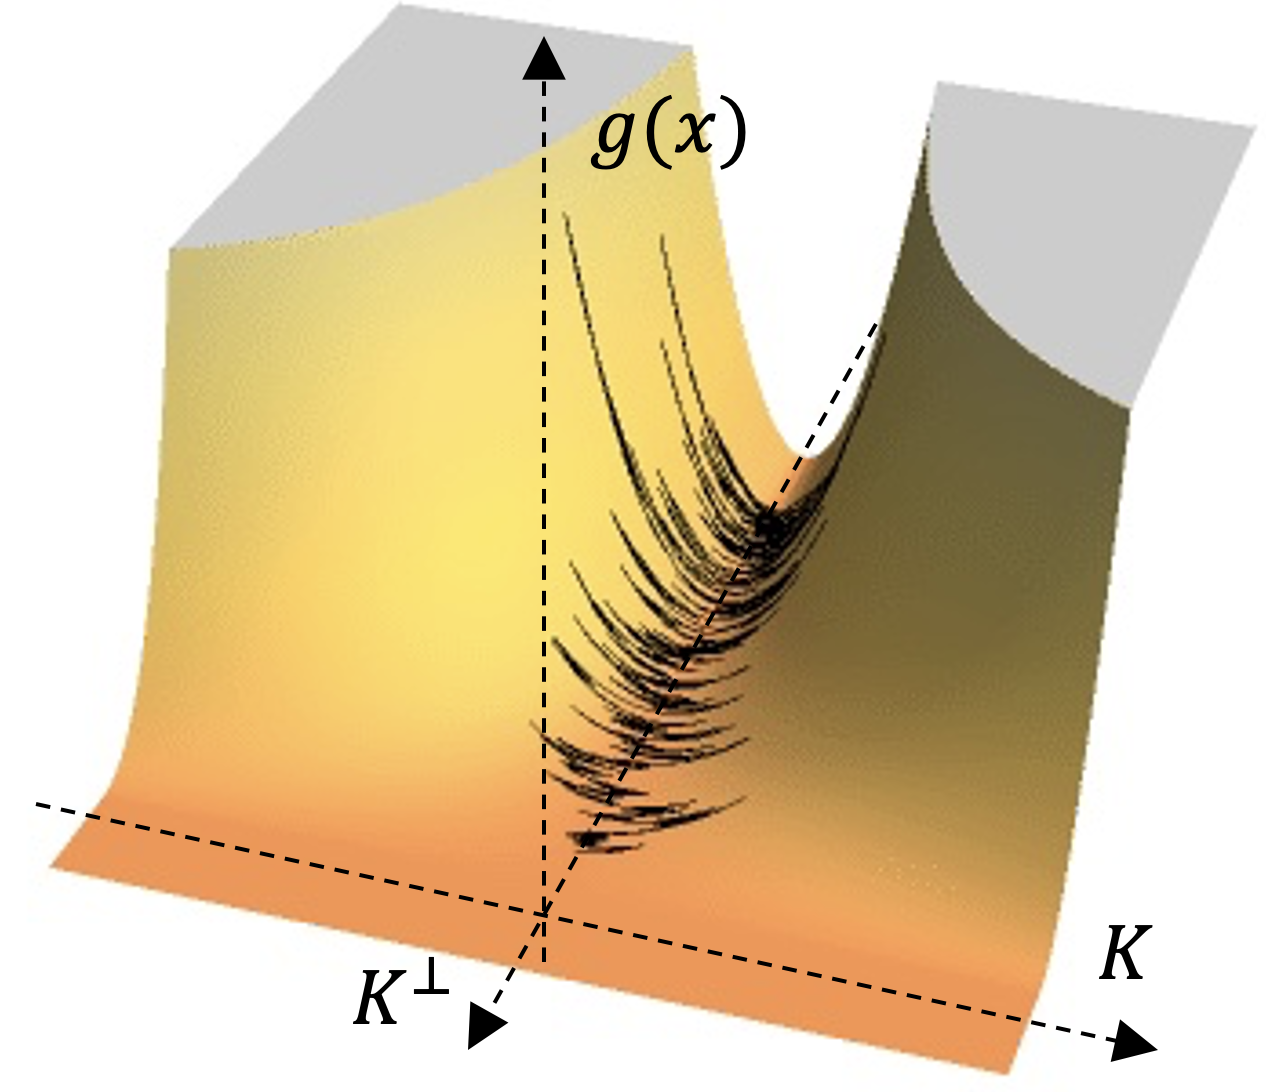
\includegraphics[width=0.50\textwidth]{figures/labelnoise-static.png}
\centering
\caption{The effect of SGD noise on non-quadratic functions. $K$ is the span of the noise covariance $\Sigma$. In the quadratic case, the iterates will fluctuate in $K$, but remains unchanged in $K^\perp$. When the function is non-quadratic, the third order effect slowly accumulates in $K^\perp$, resulting in implicit regularization. } 
\label{lec17:fig:noise}
\end{figure}

\tnote{need to add figures. I added two figures labelnoise-static.jpg and bias2.png. Also need to refer to this figure in the main texts. I did discuss in length these figures so there should be some paragraphs about these figures. }

\paragraph{Interpretation.} Intuitively, the direction of the implicit regularization is $T(S) = \nabla_x \left(\langle\nabla_x^2g(0), S\rangle\right)$. In other words, the implicit bias $-T(S)$ is trying to make $\langle\nabla^2_x g(0), S\rangle$ small. \cite{damian2021label} further prove that SGD with label noise on loss $\hat{L}(\theta)$ converges to a stationary point of the regularized loss $\hat{L}(\theta) + \lambda \textup{tr}(\nabla^2_\theta \hat{L}(\theta))$. In the next subsection, we will heuristically explain why this regularization term is useful.


\subsec{SGD with label noise}
We previously claimed that SGD with label noise minimizes the regularized loss 
\begin{equation}
    \hat{L}(\theta) + \lambda \textup{tr}(\nabla^2_\theta \hat{L}(\theta)).
\end{equation} 

But why is $\textup{tr}(\nabla^2_\theta \hat{L}(\theta))$ a useful regularizer? This question has been the subject of recent study in the implicit regularization literature. \cite{wei2019improved} show that the complexity of neural networks can be controlled by its Lipschitzness. Indeed, we will see that $\textup{tr}(\nabla^2\hat{L}(\theta))$ is intimately related to the Lipschitzness of the networks. \cite{foret2020sharpness} also discover empirically that regularizing the sharpness of the local curvature leads to better generalization performance on a wide range of tasks. In the sequel, we will unpack some of these arguments to justify regularizing by $R(\theta) \defeq \textup{tr}\left (\nabla^2 \hat{L}(\theta) \right )$.

We first consider the case of one data point, i.e. $\hat{L}(\theta) = \ell(f_\theta(x), y)$. For notational simplicity, let $f \defeq f_{\theta}(x)$ denote the model output, $p$ be the number of parameters, and $\ell(f,y)$ be the loss function. Then,
\begin{align}
    \nabla^2\hat{L}(\theta) &= \nabla_\theta \left(\diffp{\ell}{f}  \cdot \diffp{f}{\theta}\right) \\
    &= \nabla_\theta \left(\diffp{\ell}{f} \cdot \nabla_\theta f_\theta(x) \right) \\
    &= \diffp[2]{\ell}{f} \cdot \nabla_\theta f_{\theta}(x)\nabla_\theta f_{\theta}(x)^\top + \diffp{\ell}{f}\underbrace{\nabla_\theta^2 f_{\theta}(x)}_{\in \R^{p \times p}}.
\end{align}
Suppose the loss function is $\ell(f,y) = \frac{1}{2}(f-y)^2$. Then, observing that $\ell$ is simply a quadratic function of $f$, we have
\begin{align}\label{lec18:eq:gn-decom}
    \nabla^2\hat{L}(\theta) = 1 \cdot \nabla_\theta f(x) \nabla_\theta f_\theta(x)^\top + (f-y)\cdot\nabla^2_\theta f_\theta (x),   
\end{align}
Note that the first term of \eqref{lec18:eq:gn-decom} is positive semi-definite (PSD), while the second term is not necessarily PSD. In general, \eqref{lec18:eq:gn-decom} is referred to as the Gauss-Newton decomposition. Note also that for convex losses $\ell$, 
\begin{align}
    \diffp[2]{\ell}{f} \geq 0,
\end{align}
which further implies that
\begin{align}
    \diffp[2]{\ell}{f}\nabla f_\theta (x) \nabla f_\theta (x)^\top \succcurlyeq 0.   
\end{align}

Empirically, we observe that the second term $(f-y)\nabla^2f_{\theta}(x)$ is generally smaller. This is especially evident when $\theta$ is at a global minimum for which $\ell(f_\theta, y) = 0$. In this case, $(f-y)\nabla^2f_{\theta}(x)=0$ because $f_{\theta}(x)=y$. These two observations suggest that we can ignore the second term. In that case,
\begin{align}
    \mathrm{tr}\l (\nabla^2\hat{L}(\theta) \r ) &\approx \diffp[2]{\ell}{f} \cdot \mathrm{tr}\l (\nabla f(x)\nabla f(x)^\top\r ) \\
    &=\diffp[2]{\ell}{f} \cdot \norm{\nabla  f_{\theta}(x)}_2^2
\end{align}
Thus, minimizing $\mathrm{tr}\l (\nabla^2\hat{L}(\theta)\r )$ is approximately equivalent to minimizing the Lipschitzness of the model output with respect to $\theta$, which is approximately equivalent to minimizing the Lipschitzness of the model output with respect to hidden variables.

For example, let $\theta = (w_1, \dots, w_r)$, then we have 
\begin{align}
    \diffp{f}{{w_i}} = \diffp{f}{{h_{i+1}'}} \cdot h_i^\top,
\end{align}
where $h'_{i+1} = w_i h_i$, and $h_i$ denotes the hidden variables of the $i$-th layer and  $h'_{i+1}$ is the pre-activation of the $(i+1)$-th layer. Then,
\begin{align}
    \l \|\diffp{f}{{w_i}}\r \|_F = \l \|\diffp{f}{{h_{i+1}}}\r \|_2\cdot \|h_i\|_2.
\end{align}
This validates our claim that minimizing the Lipschitzness of the model output with respect to the parameters is (approximately) equivalent to minimizing the Lipschitzness of the model output with respect to the hidden variables. We have previously connected the latter concept to generalization of deep neural networks. See Section~\ref{sec:all_layer_margin} for a discussion of the all-layer margin, a measure of Lipschitzness of the model with respect to hidden layer variables that can be directly used to bound generalization error of a deep net.